
In diesem Abschnitt wird die stetige und diskrete Wavelet-Transformation betrachtet. Dabei soll ein Überblick über von Vor- und Nachteile der Wavelet-Transformation zu Frequenz-Zeit-Spektrum analyse geschaffen werden. 



\subsection{Stetige Wavelet-Transformation} 
In Kapitel \ref{chapter:cwt} wurde die Theorie der stetigen Wavelet-Transformation, auch cwt genannt, behandelt. In dieser Theorie haben wir gesehen, dass wir mit der stetigen Wavelet-Transformation eine Zeit-Frequenz-Analyse machen können, welche uns gut interpretierbare Egebnisse liefert. Der Nachteil bei der cwt ist jedoch die grosse Redundanz. Diese Redundanz spiegelt sich in der Analysedauer wieder, welche schon bei simplen Datensätzen mehrere Sekunden dauern kann, weshalb die cwt für eine realtime Applikation nicht geeignet ist.\\
Um dennoch zu zeigen welche Vorteile eine cwt bringen kann, wurde noch einmal der Frequenzsweep der Abbildung \ref{fig:stftsig} mit einem komplexen Gauss Wavelet analysiert. Das komplexe Gauss-Wavelet ist wie folgt definiert:
\begin{equation}
\psi(t)=C \cdot e^{-it} e^{-t^{2}}
\label{eq:cgau}.
\end{equation}
Bei $C$ handelt es sich um eine Konstante. Das Wavelet wurde in der folgenden Analyse in der achten Ableitung verwendet. In der Python Library wird dies mit $\texttt{cgau}N$ benannt. \text{N} steht dabei für die Häufigkeit der Ableitungen der Waveletfunktion.\\

Alle Wavelet-Transformationen wurden mit der Python Library pywt \cite{Lee2019PyWavelets} durchgeführt. Pywt stellt schon eine cwt- und viele weitere Waveletfunktionen bereit. In der Abbildung \ref{fig:python-cwt} ist ein wesentlicher Ausschnitt aus dem Python Code dargestellt, mit dessen Hilfe die cwt jeweils erstellt wurde. Da es sich um ein komplexes Wavelet handelt, wurden zur besseren Illustration der Resultate die Absolutwerte der Transformation verwendet.\\

\begin{figure}[!ht]
	\centering
	\lstinputlisting[language=Python,firstline=9,lastline=26,numbers=left,style = Python]{papers/autotune/sections/frequenzanalyse/code/cwt.py}
	\caption{Python cwt Beispiel}
	\label{fig:python-cwt}
\end{figure}

Das Ergebnis der cwt, die auf $x_{\text{sweep}}(t)$ in Abbildung \ref{fig:stft-sig} angewendet wurde, ist in der Grafik \ref{fig:cwt-sweep} ersichtlich. Dabei stehen sich eine STFT ()Abbildung \ref{fig:stft-4096}) und cwt (Abbildung\ref{fig:cwt-sweep}) gegenüber. Es ist zu beachten, dass dieser Vergleich in der Grafik \ref{fig:STFTCWT} in keinster Weise eine allgemeingültige Aussage über diese zwei Arten der Zeit-Frequenz-Analyse sein soll, sondern mehr eine Gegenüberstellung zur Betrachtung von Unterschieden. \\


\begin{figure}[!ht]
	\centering
	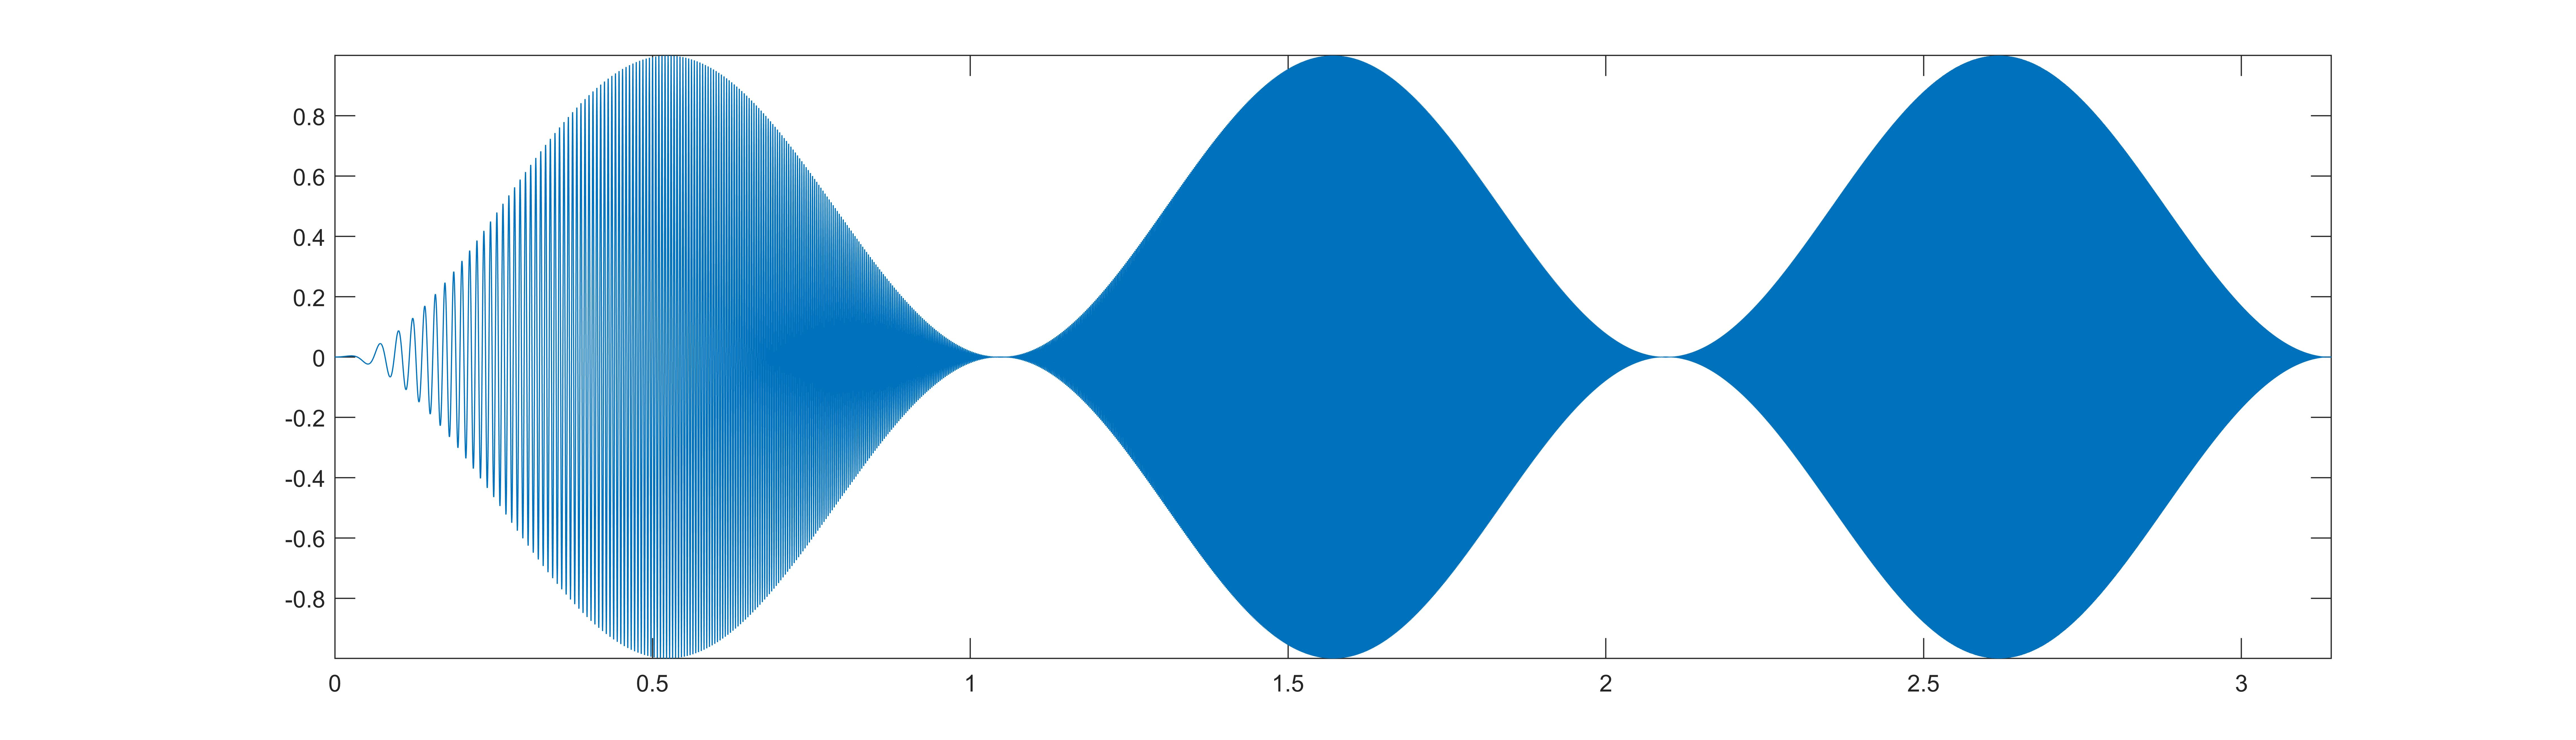
\includegraphics[width=\linewidth]{papers/autotune/sections/fft/signal.jpg}
	\captionof{figure}{Sweep Signal 0-400\text{[Hz]}}\label{fig:stft-sig}
	\begin{tabularx}{\columnwidth}{XX}
		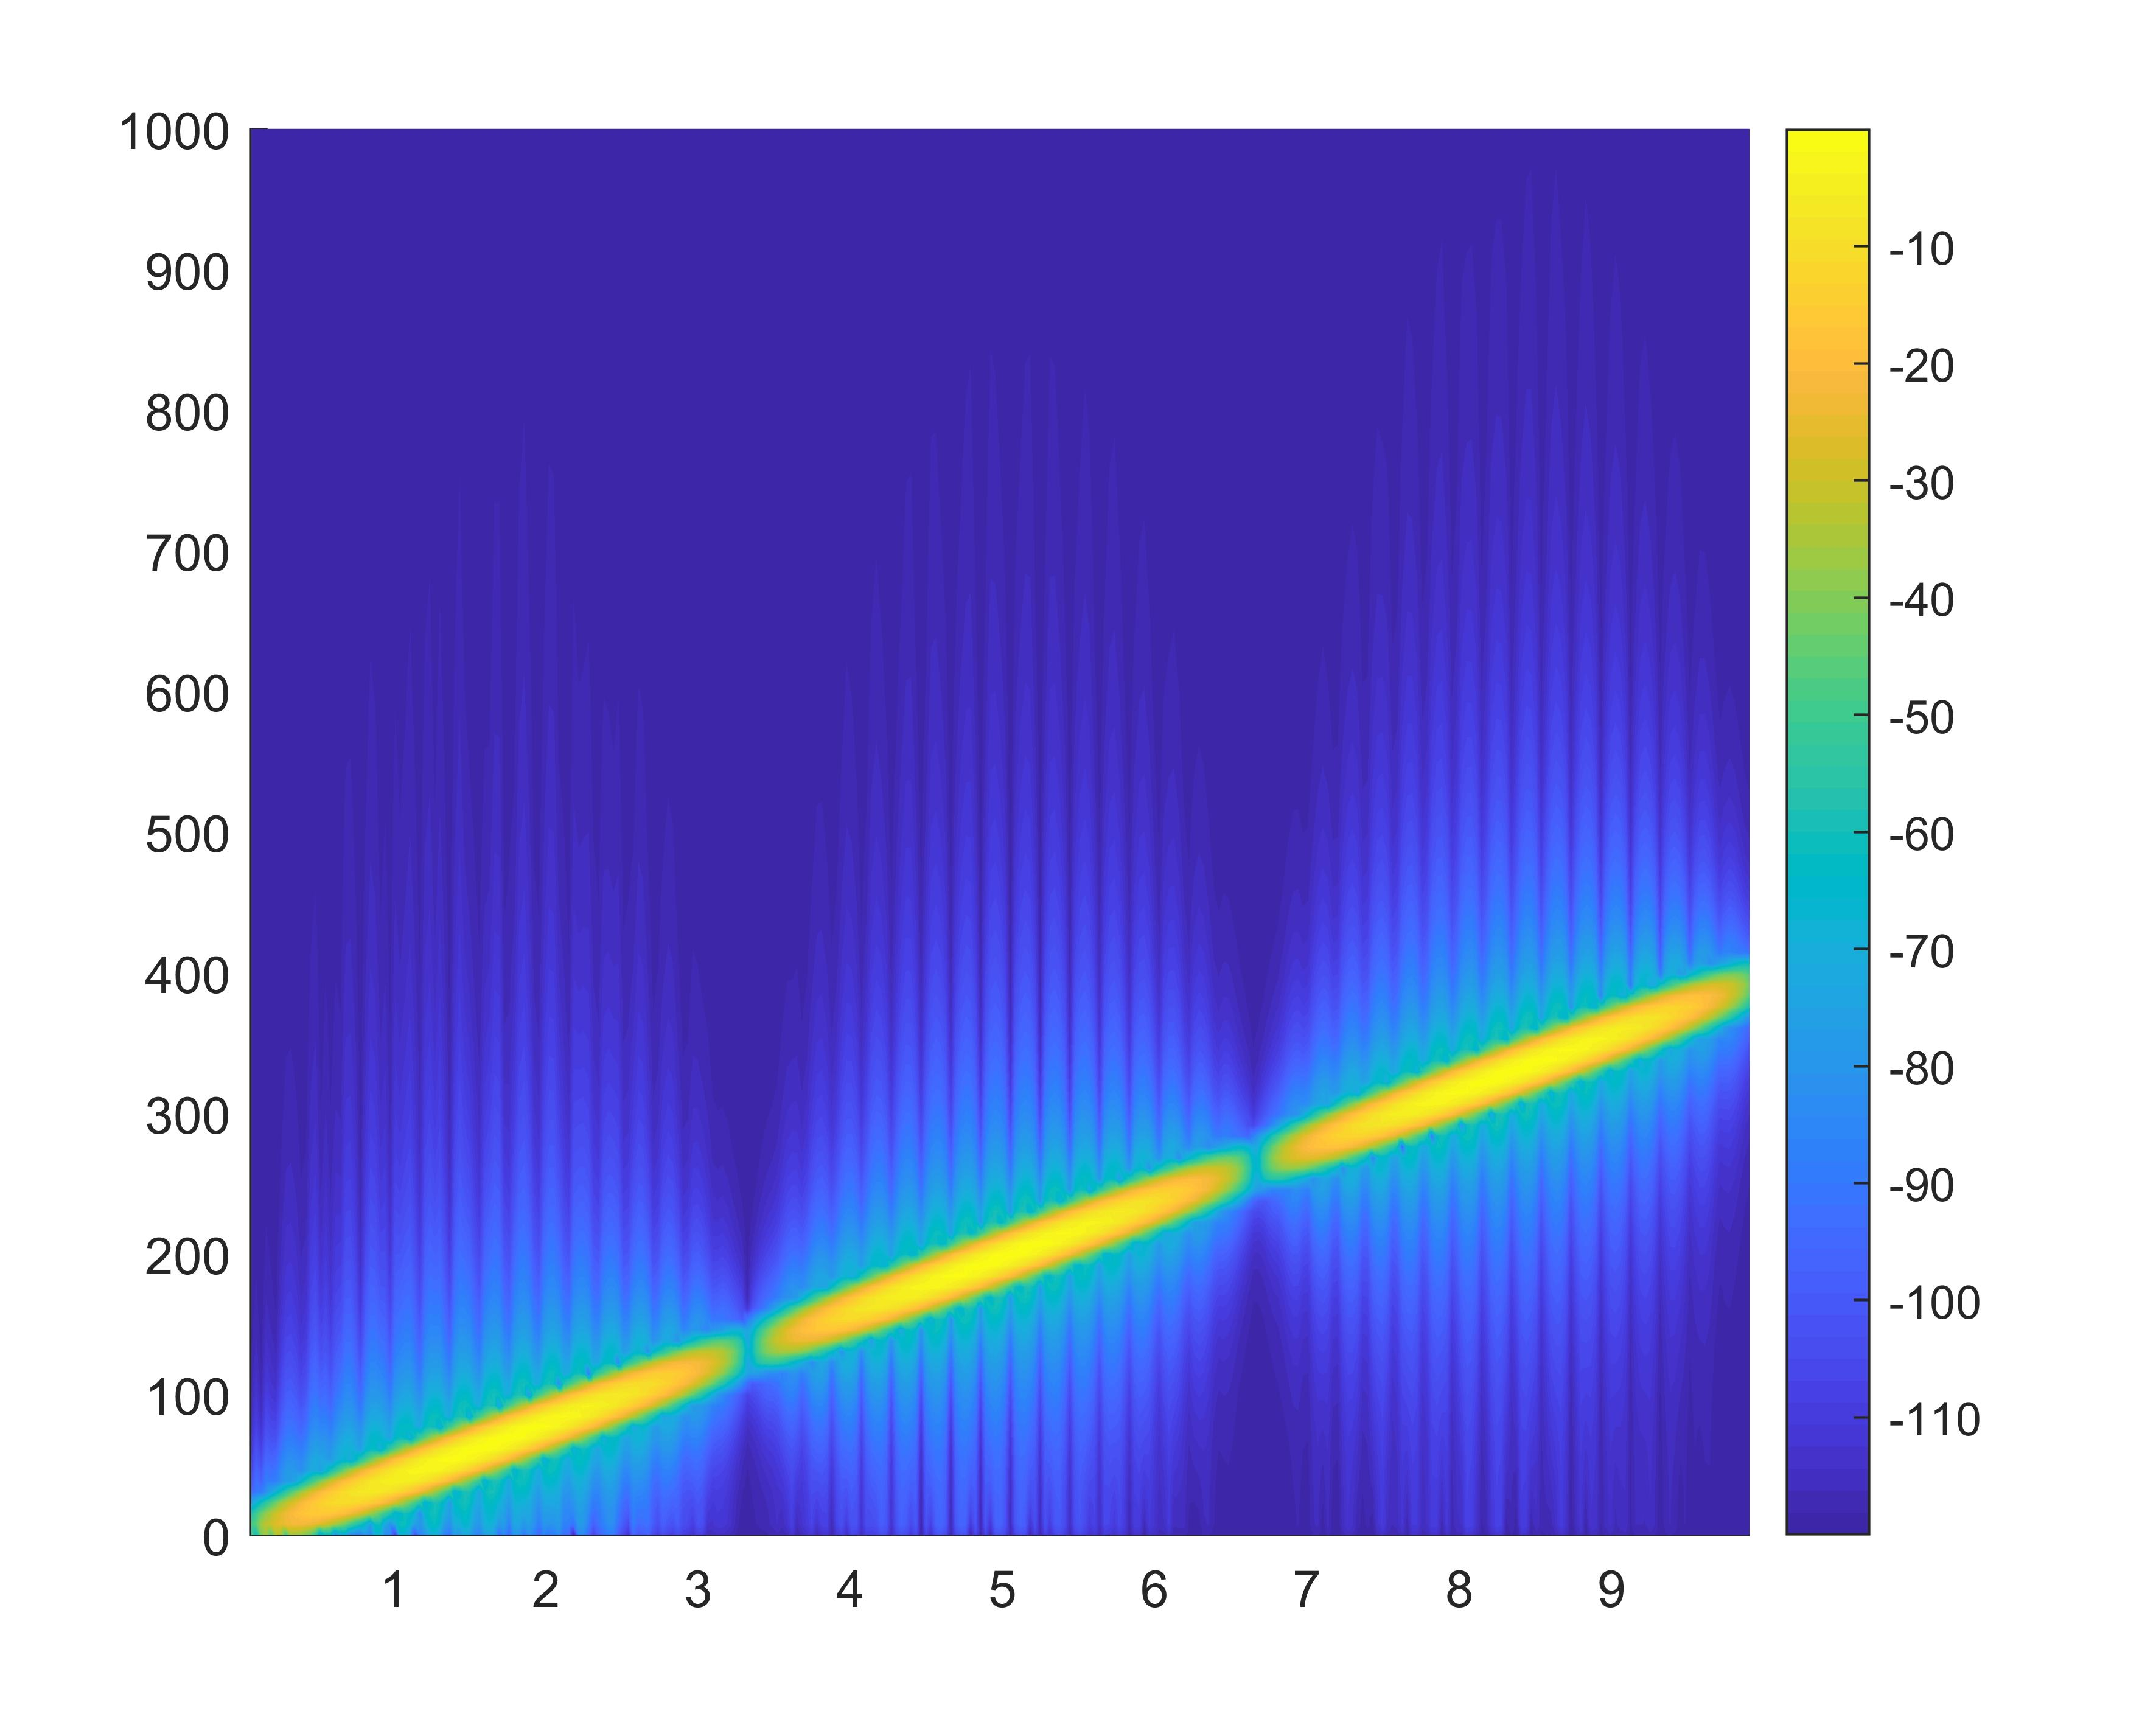
\includegraphics[width=\linewidth]{papers/autotune/sections/fft/stft4096.jpg}
		\captionof{figure}{STFT Blackman mit 4096 Sample Fenster}\label{fig:stft-4096}
		&   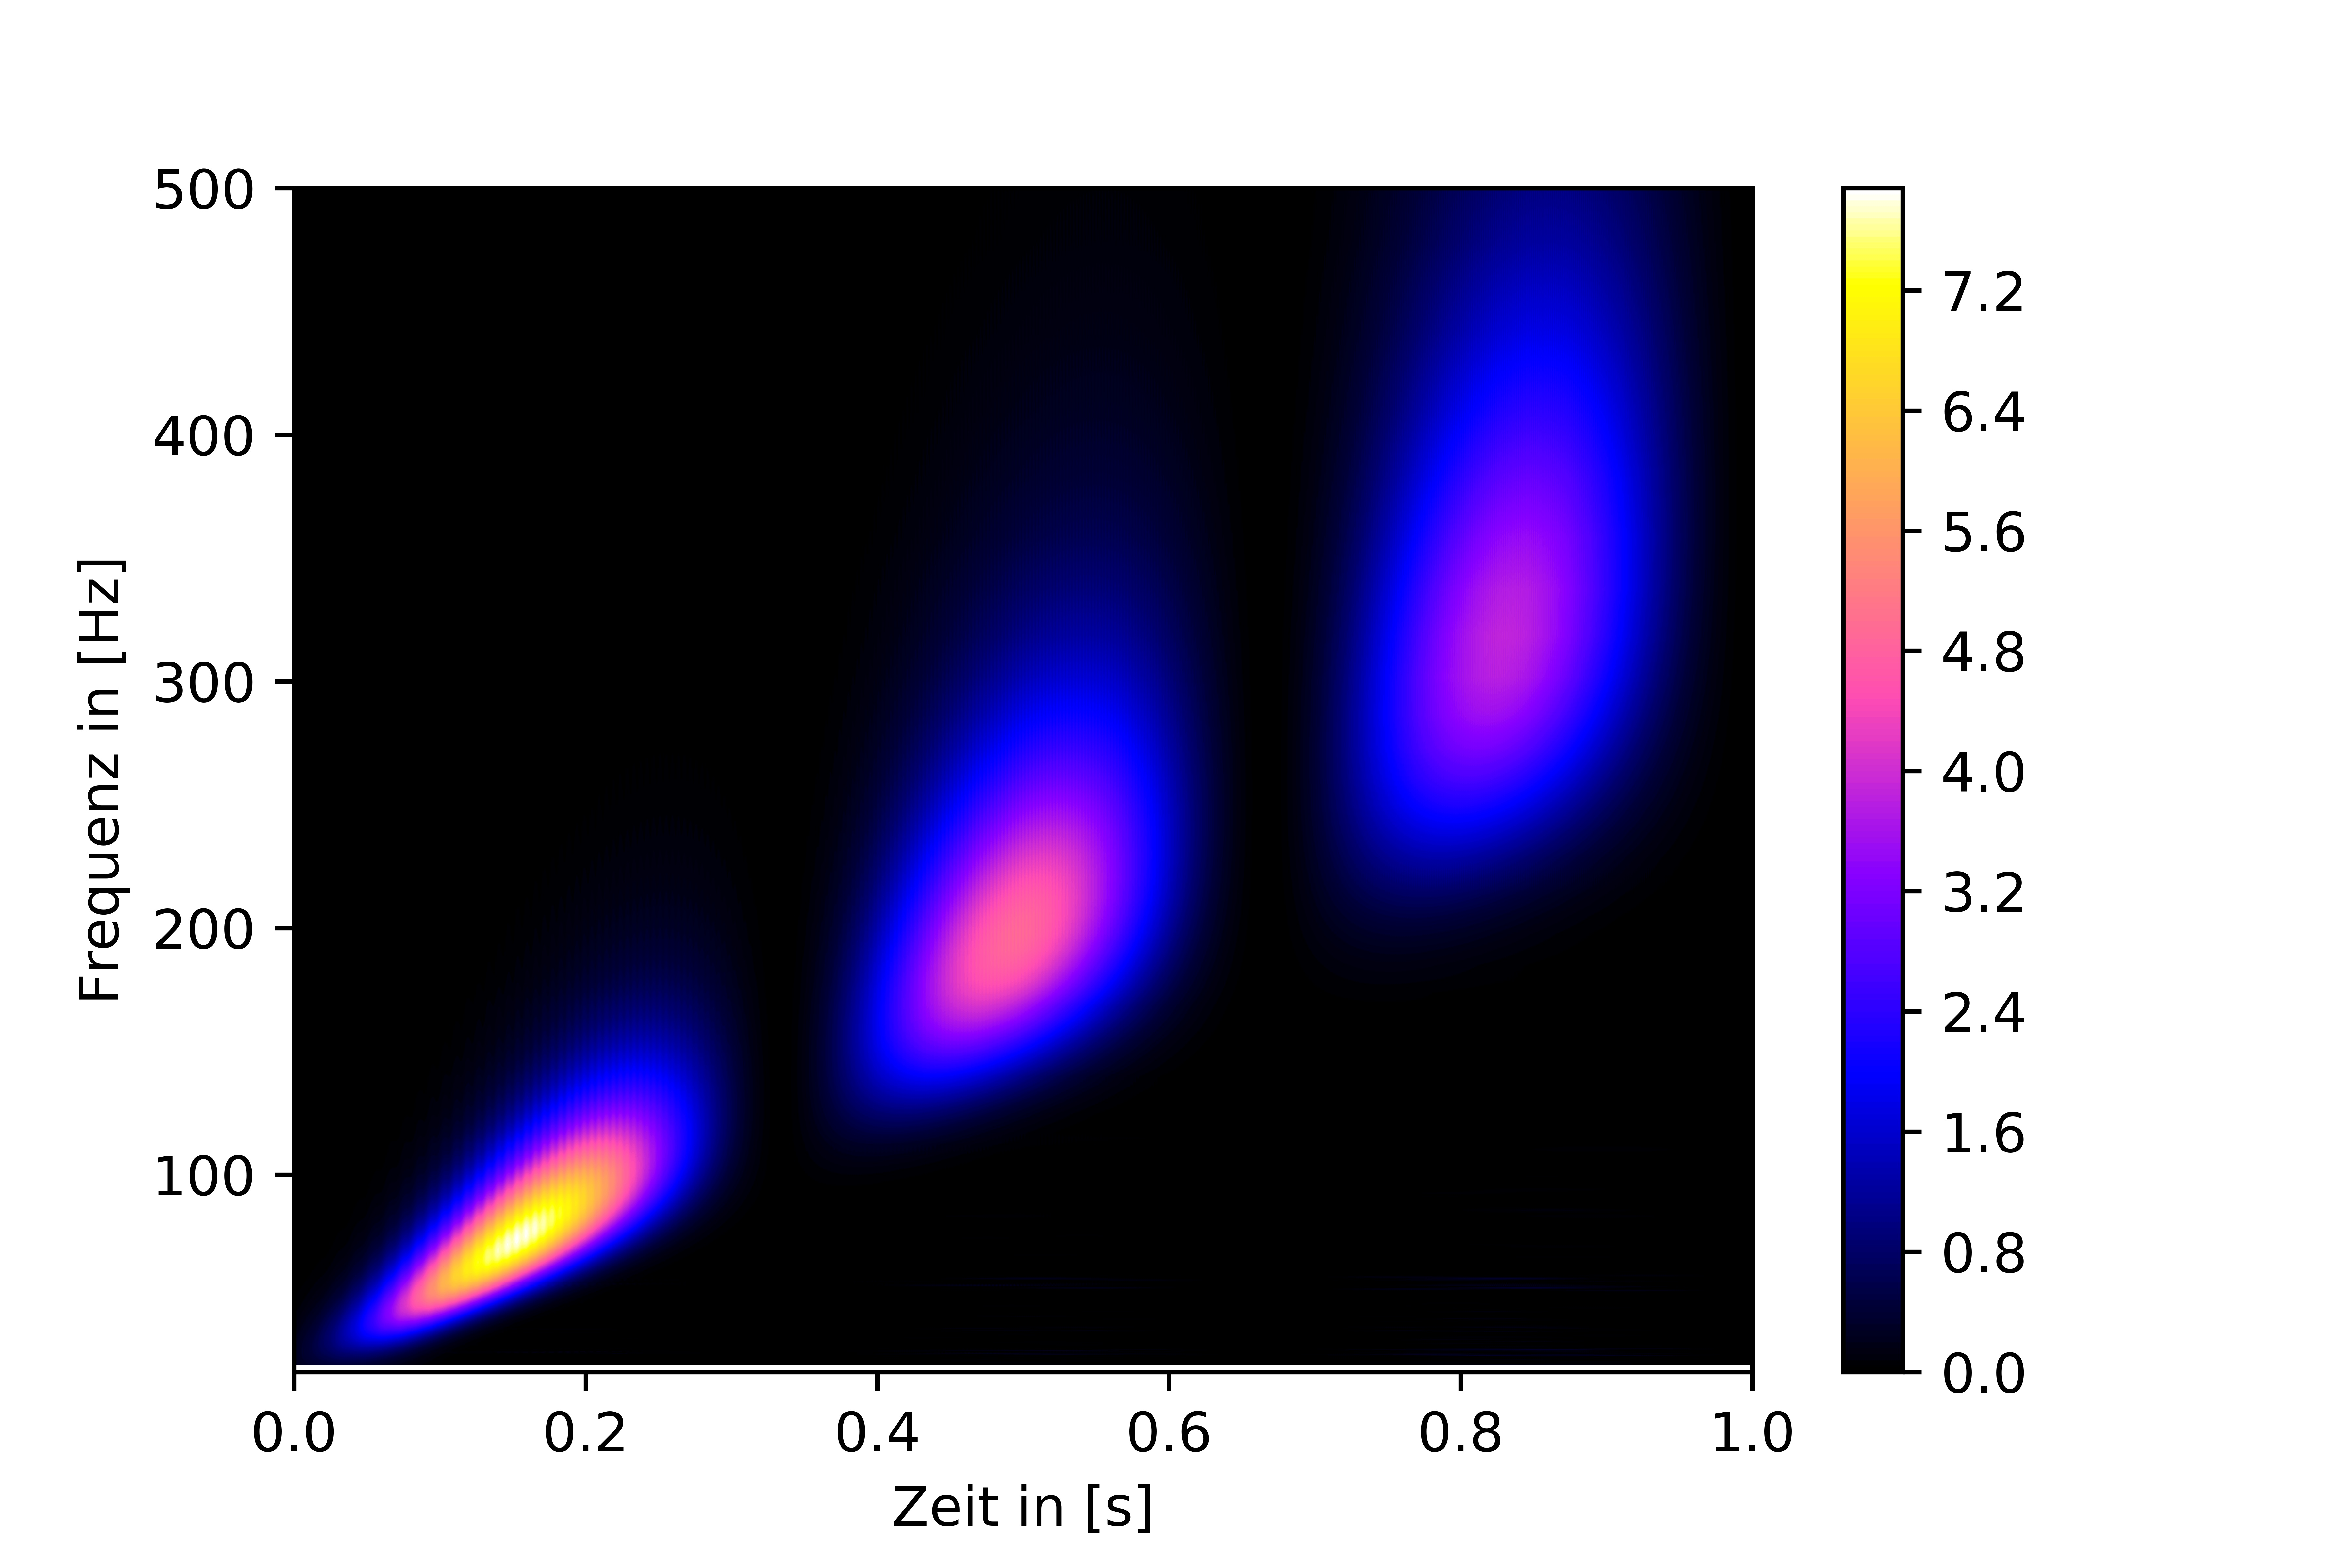
\includegraphics[width=1.24\linewidth]{papers/autotune/sections/frequenzanalyse/images/sinsweep.jpg}   
		\captionof{figure}{Komplex Gauss 8 \ref{eq:cgau} Cwt Analyse des Frequensweeps}\label{fig:cwt-sweep}         
	\end{tabularx}
	\caption{figure}{Vergleich zwischen STFT und der CWT}
	\label{fig:STFTCWT}
\end{figure}%


\subsection{Diskrete Wavelet-Transformation}
 Um eine diskrete Wavelet-Transformation über mehrere Skalen zu berechnen, bietet sich der schnelle Multiskalenanalyse-Algorithmus an. Dieser wurde genauer im Kapitel \ref{chapter:msa} behandelt. In den folgenden Teilen dieser Arbeit wurde vermehrt mit der Multiskalenanalyse gearbeitet. Für Berechnungen wurde erneut die Python pywt Library verwendet. Für die Multiskalenanalyse wurde dabei immer die Funktion \texttt{wavedec()} verwendet. Für die Auswertungen der Analyse ist jedoch die Erkenntnis ausschlaggebend, dass nur Frequenzen verwendet werden die das $2^n$-fache einer Grundfrequenz sind. Die Analyse kann also nur Oktaven unterscheiden. Dabei sind Töne einer Tonleiter im Frequenzverhältnis von $\sqrt[12]{2}$. Wir können also mit einer normalen Multiskalenanalyse nicht einzelne Töne eines Signales unterscheiden. Dennoch können wir gewisse Vorteile nutzen, wie z.B. das automatische Fenstern einer Multiskalenanalyse, wobei die Mutiskalenanalyse eine $2^n$-fache Fensterungseigenschaft besitzt. In der folgenden Grafik\ref{fig:faauf} ist die Zeit-Frequenz-Fensterung der Multiskalenanalyse neben der STFT Fensterung aufgezeigt. 
 


\begin{figure}[!ht]
	\centering
	\scalebox{0.9}{
		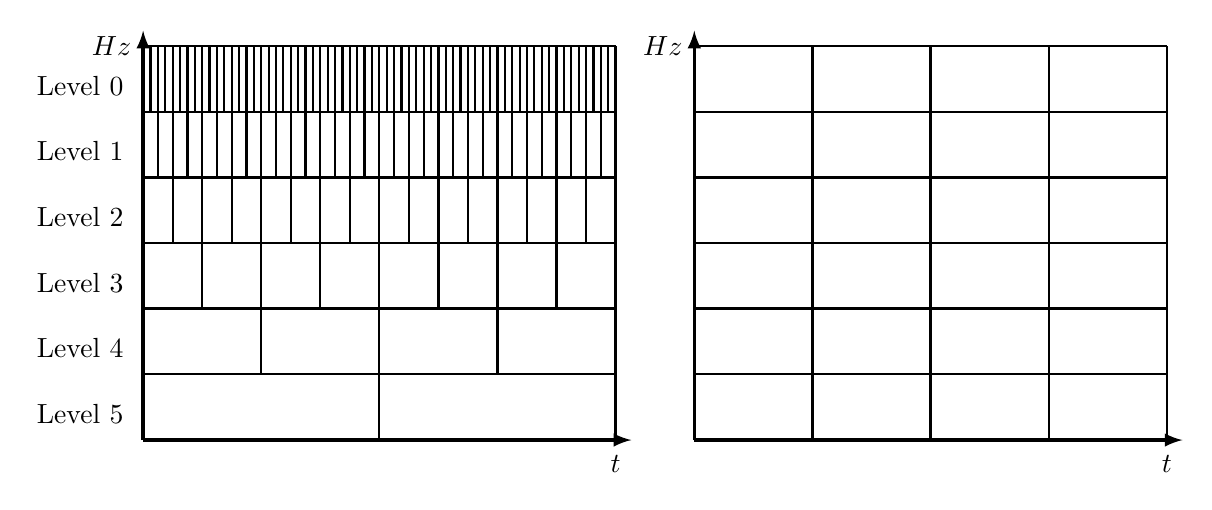
\begin{tikzpicture}[>=latex]
		\draw (6,-5.3) node{$t$};
		\draw (-0.4,0) node{$Hz$};
		
		\draw (-0.8,-0.5) node{Level 0};
		\draw (-0.8,-1.333) node{Level 1};
		\draw (-0.8,-2.166) node{Level 2};
		\draw (-0.8,-2.999) node{Level 3};
		\draw (-0.8,-3.832) node{Level 4};
		\draw (-0.8,-4.665) node{Level 5};
		
		
		\draw[->, very thick] (0,-5)--(0,0.2);
		\draw[->, very thick] (0,-5)--(6.2,-5);
		
		\draw[thick] (0,-0)--(6,-0);
		\draw[thick] (0,-0.833)--(6,-0.833);
		\draw[thick] (0,-1.666)--(6,-1.666);
		\draw[thick] (0,-2.499)--(6,-2.499);
		\draw[thick] (0,-3.33)--(6,-3.33);
		\draw[thick] (0,-4.166)--(6,-4.166);
	
		\draw[thick] (3,-5)--(3,0);
		\draw[thick] (6,-5)--(6,0);
		\draw[thick] (1.5,-4.166)--(1.5,0);
		\draw[thick] (4.5,-4.166)--(4.5,0);
		
		\draw[thick] (0.75,-3.33)--(0.75,0);
		\draw[thick] (2.25,-3.33)--(2.25,0);
		\draw[thick] (3.75,-3.33)--(3.75,0);
		\draw[thick] (5.25,-3.33)--(5.25,0);
		
		\foreach \x in {0,0.375,...,6}
			\draw[thick] (\x,-2.499)--(\x,0);
		
		\foreach \x in {0,0.1875,...,6}
			\draw[thick] (\x,-1.666)--(\x,0);
		
		\foreach \x in {0,0.09375,...,6}
			\draw[thick] (\x,-0.833)--(\x,0);
		
		\draw (13,-5.3) node{$t$};
		\draw (6.6,0) node{$Hz$};
		\draw[->, very thick] (7,-5)--(7,0.2);
		\draw[->, very thick] (7,-5)--(13.2,-5);
		
		\draw[thick] (7,-0)--(13,-0);
		\draw[thick] (7,-0.833)--(13,-0.833);
		\draw[thick] (7,-1.666)--(13,-1.666);
		\draw[thick] (7,-2.499)--(13,-2.499);
		\draw[thick] (7,-3.33)--(13,-3.33);
		\draw[thick] (7,-4.166)--(13,-4.166);
		
		\draw[thick] (8.5,-5)--(8.5,0);
		\draw[thick] (10,-5)--(10,0);
		\draw[thick] (11.5,-5)--(11.5,0);
		\draw[thick] (13,-5)--(13,0);
		\end{tikzpicture}
	}
	\caption{Multiskalenanalyse-Fensterung im Vergleich zu STFT-Fensterung}\label{fig:faauf}
	
\end{figure}

Wie man in der Abbildung \ref{fig:faauf} erkennt, übernimmt die Multiskalenanalyse, folgend auch msa abgekürzt, das Fenstern. Dabei geht die Wavelet-Transformation einen Kompromiss ein. Im oberen Bereich, wo die höheren Frequenzen liegen, sieht man den Zeitpunkt sehr genau. Die tieferen Frequenzen werden dabei wie bei einem Hochpass weggefiltert. In den tieferen Levels erkennt man die tiefen Frequenzen, jedoch sind diese nicht mehr sehr genau auf dem Zeitstrahl abgebildet. Gerade bei der Multiskalenanalyse können durch tiefe Frequenzen an den Rändern oder bei den Unstetigkeiten eines Signales, Artefakten enstehen. In der Grafik \ref{fig:faauf} können die beiden Darstellungen der Zeit-Frequenzaufteilung von der STFT und Multiskalenanalyse nicht direkt miteinander verglichen werden. Die Grafiken sind dafür nicht richtig skaliert. Sie dienen lediglich zur sinnbildlichen Darstellung in dessen Aufteilung.

Um die $2^{n}$-fache Fensterung zu verdeutlichen, wird eine  Multiskalenanalyse des weiter oben verwendeten Sinussweeps (Abbildung \ref{fig:STFT}) gemacht und gleich mit der STFT verglichen.
Die msa wird mit einem Daubechies 8 Wavelet durchgeführt. Die verwendete Daubechies-Familie ist in der tabellarischen Abbildung \ref{tab:Daubechies} zu finden. Eine Multiskalenanalyse kann nicht mit dem gleichen Wavelet durchgeführt werden wie die cwt. Der Grund dafür ist, dass in der Python pywt Library die stetigen und diskreten Wavelets getrennt sind und es keine Überlappungen gibt.

In dieser Tabelle \ref{tab:Daubechies} werden vier verschiedene Daubechies Wavelets, in verschiedener Auflösung, dargestellt. Dabei handelt es sich um die numerisch berechneten Vater und Mutter Wavelets. Auch wird gut ersichtlich, dass die höheren Daubechiesfunktionen mehr Samples brauchen um korrekt dargestellt zu werden. Zur Berechnung der Koeffizienten wird auf das Kapitel \ref{section:daubechies} verwiesen.


\begin{table}[!ht]
	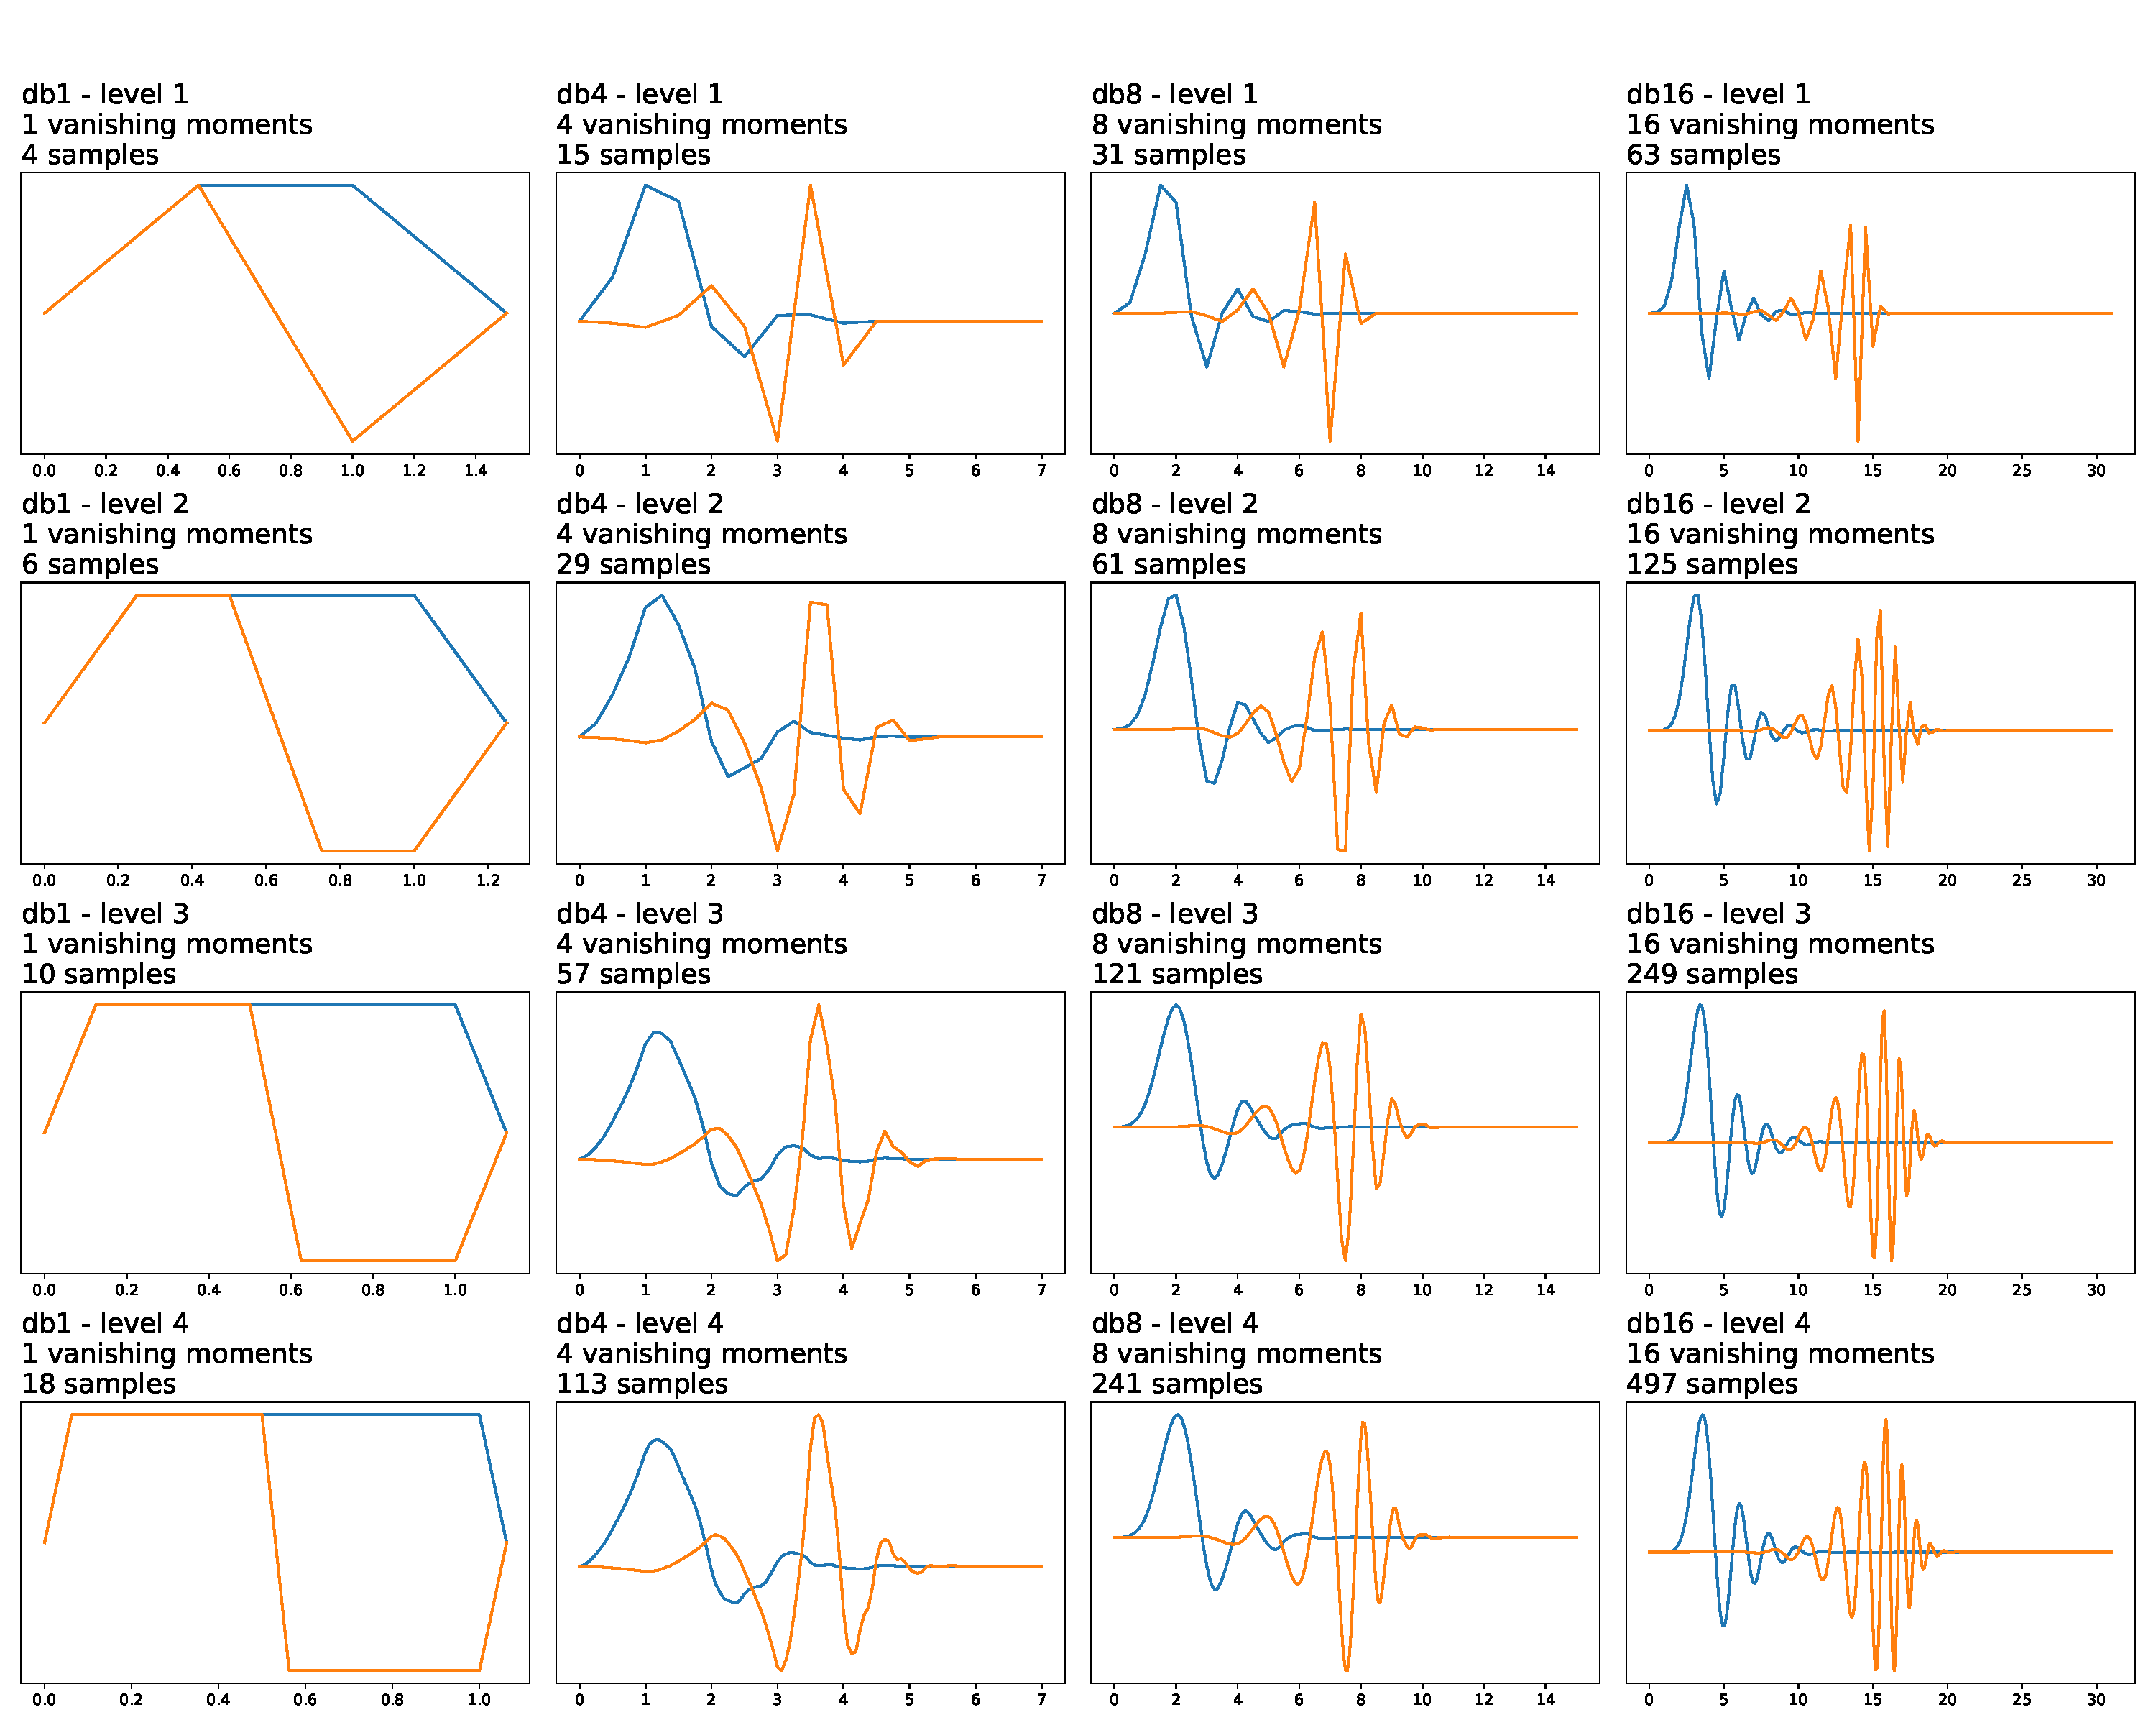
\includegraphics[width=\linewidth]{papers/autotune/sections/frequenzanalyse/images/DaubechiesFamilie.pdf}
	\caption{Eine kleine Auswahl aus der Daubechies Familie}
	\label{tab:Daubechies}
\end{table}

Das Ergebnis der Multiskalenanalyse ist in der Grafik \ref{fig:sin-sweep} wiedergegeben. Im Frequenzbereich sieht man eine klare Verschlechterung im Vergleich zur cwt Analyse  \ref{fig:STFTCWT}. Nur die jeweiligen Oktaven sind erkennbar. Für eine genauere Frequenz-Analyse sind diese Ergebnisse jedoch unbrauchbar.  


\begin{figure}[!ht]
	\centering
	\includegraphics[width=\linewidth]{papers/autotune/sections/frequenzanalyse/images/sweepdwt.jpg}
	\captionof{figure}{Diskrete Wavelet Analyse des Sinus Sweep 0-400$Hz$}\label{fig:sin-sweep}
\end{figure}%




